\documentclass[a4paper]{llncs}
%

% Additional packages used
\usepackage[utf8]{inputenc}
\usepackage[portuges]{babel}
\usepackage{hyphenat}
\usepackage{amsmath}
\usepackage[pdftex]{graphicx}
\usepackage{tabularx}
\usepackage{comment}
\usepackage{calc}
\usepackage{pslatex}
\usepackage{listings}
\usepackage{url}
\usepackage{caption}
\usepackage{subcaption}
\usepackage{footnote}
\usepackage{float}
\captionsetup{compatibility=false}

% Packages needed for the table with alternating colors
\usepackage{xcolor}
\usepackage{colortbl}
\usepackage{booktabs}
\usepackage{tabu}

% Enumeration item customization
% \usepackage{enumitem}

% Inline lists
\usepackage{paralist}

%%%%%%%%%%%%%%%%%%%%%%%%%%%%%%%%%%%%

\newcommand{\alternativa}[1]{}
\newcommand{\ie}{\textit{i.e.},\ }
\newcommand{\eg}{\textit{e.g.},\ }
\newcommand{\etal}{\textit{et al.}\ }
\newcommand{\cf}{\textit{c.f.}\ }
\newcommand{\mapenc}{\textit{Map/Encap}}
\newcommand{\map}{sistema de \textit{mapping}}
\newcommand{\discutir}{\textbf{[por discutir] \ \ \ \ $\rightarrow$\ \ \ \ }}
\newcommand{\loc}{lo\-ca\-li\-za\-ção}



\newcommand{\lincont}{\textit{linux container }}
\newcommand{\cont}{\textit{container}}
\newcommand{\conts}{\textit{containers}}
\newcommand{\Cont}{\textit{Container}}
\newcommand{\Conts}{\textit{Containers}}
\newcommand{\cloud}{\textit{cloud}}
\newcommand{\clouds}{\textit{clouds}}


%%%%%%%%%%%%%%%%%%%%%%%%%%%%%%%%%%%%

% Adjust distance between floats (figures and tables) and text
% \setlength{\belowcaptionskip}{-10pt}
% \setlength{\abovecaptionskip}{-10pt}

%%%%%%%%%%%%%%%%%%%%%%%%%%%%%%%%%%%%

\begin{document}

\title{{\Conts} versus Máquinas Virtuais para Emulação de Controlo de Redes}
\author{Bruno Anjos, Nuno Morais, Paulo Lopes e Jos\'{e} Legatheaux Martins}
%%%% list of authors for the TOC (use if author list has to be modified)
\tocauthor{}

\institute{NOVA LINCS, Departamento de Informática\\
           Faculdade de Ciências e Tecnologia, Universidade Nova de Lisboa\\
           2829--516 Caparica, Portugal\\
%
           \email{ \{b.anjos@campus., nm.morais@campus, paulo.lopes, jose.legatheaux\}@fct.unl.pt} \\
           \url{http://di.fct.unl.pt}
           }


%\keywords{}

\maketitle              % typeset the title of the contribution


\begin{abstract}
Dada a complexidade e as dificuldades associadas ao teste de
protocolos distribuídos para controlo de equipamentos de rede num
contexto real, é comum recorrer a emulação para teste dos mesmos. Os
primeiros emuladores recorriam a máquinas reais, interligadas através
de um sistema de emulação do tempo de trânsito e da perda de pacotes
numa rede real [ModelNet].

Com o desenvolvimento das tecnologias de virtualização, seja esta através de
máquinas virtuais ou de \conts, tornou-se atractivo substituir as
máquinas reais e os equipamentos de comutação por sistemas
virtualizados. Um dos sistemas mais populares que seguem esta
abordagem é o sistema MiniNet [ MiniNet ], para emulação de redes
controladas com a abordagem Software Defined Networking e o protocolo
OpenFlow. Outros sistemas, que utilizam outros protocolos e outros
tipos de equipamentos de comutação, utilizam para o mesmo efeito
máquinas virtuais [ Cisco ].

No quadro de um projecto em que se pretende testar protocolos de
controlo de equipamentos de rede mais complexos que os switches
OpenFlow, e utilizando protocolos distribuídos com semântica de falhas
bem definidas, da classe dos usados em bases de dados distribuídas,
coloca-se o problema de decidir qual a tecnologia de virtualização a
utilizar: máquinas virtuais (VMs) ou {\conts} implementados pelo sistema
Docker.

Este artigo apresenta um estudo empírico comparativo das tecnologias:
máquinas virtuais implementadas sobre o hipervisor 
ESXi da VMWare e containers Docker suportados quer no interior de VMs, quer em modo nativo.
A execução de containers no interior de VMs, parecendo um contrasenso, 
não o é de facto pois a maioria das plataformas de grande escala (e.g., \clouds)
hoje acessíveis não disponibiliza acesso nativo aos utilizadores.


\end{abstract}

\label{introducao}

\section{Introdução}

\subsection{XXXXXXXXXX }

{ \color{blue} Explicar a razão de ser do trabalho, porque foi necessário, como se fez e dar uma
breve panoramica dos resultados - usar parte do abstract que passará a ser mais resumido.}



Dada a complexidade e as dificuldades associadas ao teste de
protocolos distribuídos para controlo de equipamentos de rede num
contexto real, é comum recorrer a emulação para teste dos mesmos. Os
primeiros emuladores recorriam a máquinas reais, interligadas através
de um sistema de emulação do tempo de trânsito e da perda de pacotes
numa rede real [ModelNet].

Com o desenvolvimento das tecnologias de virtualização, seja esta através de
máquinas virtuais ou de \conts, tornou-se atractivo substituir as
máquinas reais e os equipamentos de comutação por sistemas
virtualizados. Um dos sistemas mais populares que seguem esta
abordagem é o sistema MiniNet \cite{Lantz:2010:NLR:1868447.1868466}, para emulação de redes
controladas com a abordagem Software Defined Networking e o protocolo
OpenFlow. Outros sistemas, que utilizam outros protocolos e outros
tipos de equipamentos de comutação, utilizam para o mesmo efeito
máquinas virtuais [ Cisco ].

No quadro de um projecto em que se pretende testar protocolos de
controlo de equipamentos de rede mais complexos que os switches
OpenFlow, e utilizando protocolos distribuídos com semântica de falhas
bem definidas, da classe dos usados em bases de dados distribuídas,
coloca-se o problema de decidir qual a tecnologia de virtualização a
utilizar: máquinas virtuais (VMs) ou {\conts} implementados pelo sistema
Docker.

Este artigo apresenta um estudo empírico comparativo das tecnologias:
máquinas virtuais implementadas sobre o hipervisor 
ESXi da VMWare e containers Docker suportados quer no interior de VMs, quer em modo nativo.
A execução de containers no interior de VMs, parecendo um contrasenso, 
não o é de facto pois a maioria das plataformas de grande escala (e.g., \clouds)
hoje acessíveis não disponibiliza acesso nativo aos utilizadores.

Foi então realizado um plano de trabalhos, visando definir os objectivos do projecto de investigação e estabelecer alguns \textit{deadlines} e a respectiva alocação de tempo para cada tarefa.
\vspace{5mm}

\textbf{Semana 1 (8/4/2018 : 15/4/2018)}

\begin{enumerate}
\item Automatizar o deployment da aplicação de teste para  executar múltiplos testes num quadro simples de um container por nó
\end{enumerate}

\textbf{Semanas 2 a 4 (15/4/2018 : 6/5/2018)}


\begin{enumerate}
\item Estudar as tecnologias presentes e descobrir as diferenças fundamentais entre as mesmas
\item Formular uma hipótese sobre qual a  raiz das diferenças de desempenho
\item Identificar os parâmetros e configurações a medir que permitam efetuar a comparação de resultados de forma rigorosa

\end{enumerate}

\textbf{Semana 5 a 7 (6/5/2018 : 27/5/2018)}

\begin{enumerate}
\item Definir cenários (um ou mais servidores) e parâmetros de teste
\item Executar os testes
\item Analisar os resultados obtidos
\end{enumerate}


\textbf{Semana 8 a 9 (27/5/2018 : 10/6/2018)}

\begin{enumerate}
\item Consolidar a análise dos dados obtidos
\item Elaboração do relatório
\end{enumerate}


\label{virtualizacao}

\section{Máquinas virtuais versus \conts}

{ \color{red} Bruno e Nuno vão adiantando }
{ \color{blue} Apresentação breve das duas tecnologias com pequeno esboço de comparação: }

A virtualização, nomeadamente sob a forma de Máquinas Virtuais é uma tecnologia que se encontra presente 
em múltiplos sistemas em produção. Esta tem progredido maioritariamente devido á sua vasta utilização no contexto empresarial, as primeiras ocorrências desta surgiram na década de 1960 e atualmente ainda se encontram em desenvolvimento. Num entanto, recentemente surgiram novas tecnologias de virtualização com a introdução do  \lincont em 2013. Esta nova tecnologia trouxe consigo uma solução mais leve em termos de recursos exigidos, mas à custa de uma virtualização mais fraca e uma maior dependência do sistema do \textit{host}. A vertente de emulação de containers é referida sempre num ambiente \textit{linux} com o \textit{Docker} como solução de \conts. Esta decisão é tomada visto que as soluções para Windows e macOS passam pela implementação de um hipervisor sobre o sistema operativo correspondente que, neste caso de comparação entre as duas tecnologias, não faria sentido comparar uma implementação de containers que não corresponda a todo o potencial da solução.


\subsection{Máquinas Virtuais}

Num ambiente de virtualização por recurso a máquinas virtuais, o foco principal cai sobre o hipervisor. Este é o componente fundamental que se responsabiliza por ocultar o sistema \textit{host} e disponibilizar apenas os recursos definidos à máquina virtual, virtualizando assim um subsistema do \textit{hardware} que se apresentam como os recursos disponíveis para a mesma.

\discutir{\textbf{COLOCAR TABELA????}

\subsection{\Conts } \label{section_conts}


A tecnologia dos \conts baseia-se numa virtualização ao nível do sistema de operação através dos \textit{control groups} e \textit{kernel namespaces} presentes no \textit{linux}, isto permite que várias instâncias de \conts possam ser executadas sobre o mesmo kernel, evitando assim a camada de virtualização do \textit{hardware} presente nas máquinas virtuais. Como referido anteriormente, a tecnologia Docker, utilizada como opção do ambiente de containers, domina atualmente o mercado no que toca a este tipo de virtualização. Num entanto, embora em constante progresso, a segurança destes ainda é um fator de preocupação.

\subsection{Conclusões}

Em suma as principais diferenças entre as duas opções de virtualização resumem-se no consumo e necessidade de recursos por instância, isolamento entre instâncias e no nível de abstração e independência do sistema \textit{host}. Claro que outras diferenças como por exemplo o tempo de arranque, espaço consumido em disco e até as ferramentas disponibilizadas pelos autores das tecnologias também contribuem para  as diferenças das tecnologias, ainda que não sejam fatores decisivos. Podemos então afirmar que o \textit{overhead} introduzido pelo hipervisor e pelo sistema operativo do \textit{guest} é determinante na performance, o qual não existe nos \conts, como já mencionadas em \ref{section_conts}. Apesar disto, a necessidade de isolamento entre processos em sistemas em produção é um fator crítico, talvez seja por isto que até á data (2018), a maioria dos sistemas em produção se encontram implementados num sistema de máquinas virtuais.


\subsection{XXXXXXXXXX}



\label{benchmarks}



\section{Benchmarks e metodologia de testes}

\subsection{Motivação}

O controlo de redes ao nível do chamado \emph{Control Plane} (protocolos e subsistemas responsáveis
pelo encaminhamento, gestão, optimização das redes) baseia-se, por razões relacionadas
com a necessidade de um elevado desempenho e de simplicidade, em protocolos de coordenação
entre as diferentes componentes de rede (e.g. \emph{switches, routers, controladores \dots}) com
níveis de consistência do tipo ``consistência eventual''. Por essa razão, o estado propagado ou computado
pelas diferentes componentes da rede transita entre estados consistentes,  passando por períodos de
inconsistência mais ou menos prolongados como é comum quando se utilizam protocolos como
OSPF, IS-IS,~\cite{francois2005achieving}, BGP~\cite{bgpConvergence,consensus-bgp},
OpenFlow~\cite{McKeown:2008:OEI:1355734.1355746}.

O trabalho descrito neste documento integra-se num projecto em que se procura substituir esse nível de \emph{consistência eventual}
por protocolos baseados em níveis de consistência com propriedades bem definidas e sem períodos intermédios de
inconsistência, em redes baseadas no paradigma SDN (\emph{Software Defined Networking}). Nomeadamente,
no que diz respeito aos protocolos de troca de estado, eventos e comandos entre componentes. Um dos objectivos do projecto
passa por substituir as funcionalidades em parte desempenhadas pelo protocolo OpenFlow,
por protocolos da mesma natureza que os protocolos usados para replicar estado em sistemas de bases de dados,
numa abordagem como a descrita em~\cite{dbcp}.

Dados os objectivos do projecto, e tendo em consideração que o principal obstáculo a vencer será o de
conseguir responder ao desafio de obter um desempenho adequado, a avaliação realista do desempenho, em redes de média
ou alta complexidade, é de uma grande importância. Para isso serão necessários emuladores de rede recorrendo a
virtualização, dado ser esta a forma mais realista de proceder a essa avaliação.

O sistema a emular deverá ter um elevado número de  \emph{switches, routers,} controladores \dots a
comunicarem intensamente entre si, utilizando protocolos da mesma natureza que os dos sistemas de
bases dados. Para fazer o estudo comparativo da adequação da emulação com base em máquinas
virtuais versus baseadas em {\conts}, revelou-se necessário utilizar um {\bench}
específico, com características bastante diferentes dos em que esses estudos comparativos têm geralmente lugar, \cf Secção~\ref{relacionado}.
Assim, essa aplicação de teste deve ser caracterizada por uma troca intensa de dados entre as diferentes
componentes do sistema, através de protocolos do tipo dos usados em base de dados, e
simultaneamente, executar em cada componente operações também da mesma natureza que as
requeridas pela execução de actualizações de tabelas de bases de dados.

\subsection{Descrição do \textit{benchmark}}

Visando este projecto a comparação das soluções de virtualização de um ambiente distribuído com as características atrás indicadas, foi desenhada de raiz uma aplicação representativa de um sistema dessa natureza. Como indicado na seção \ref{relacionado}, não foi possível utilizar os mesmos {\textit{benchmarks}} que são usados em estudos semelhantes. A aplicação desenvolvida baseia-se num conjunto de nós em que cada nó possui uma base de dados local. Todos os nós têm acesso à base de dados local, como também à base de dados de todos os outros.

Após uma fase de inicialização, cada nó começa a inserir tuplos nas bases de dados de todos os nós, incluindo a sua cópia local. A aplicação termina quando todos os nós tiverem na base de dados local a totalidade dos tuplos inseridos por todos os nós, os quais são necessariamente indênticos.

Ao variar o débito das inserções e o número de nós do sistema distribuído, é possível analisar a capacidade de emulação de uma rede virtual como também observar quais os limites desta.

O servidor onde foram efetuados os \textit{benchmarks} é composto por dois processadores \textit{Intel Xeon E5-2670 v3} a 2.30GHz com 24 núcleos físicos (48 lógicos) cada, 128GB de RAM DDR4 2400MHz. Este executa o {\hiper} VMWare ESXi 6.5.

Para os testes com {\conts}, foi instanciada no mesmo servidor uma VM que permite os testes correrem num ambiente semelhante a um sistema \textit{cloud}, onde os {\conts} executam sobre uma VM instanciada por questões de segurança. As especificações desta VM consistem em 24 \textit{cores} físicos (48 lógicos) e 94GB de RAM. Foi observado que o sistema, durante os testes, não saturava a memória alocada. O sistema de operação da VM onde foram executados os \textit{benchmarks} foi o CentOS 7. Nos {\conts} é usado MySQL 14.14, Python 3.5.3 e como sistema operativo o Debian 9. As versões de MySQL são distintas.

Para os testes de VMs, foram instanciadas tantas VMs quantos os números de nós parametrizados. Cada VM possuía 4 núcleos do CPU e 3 GB RAM. As ferramentas empregues foram: MySQL 15.1, Python 3.4.8 e como sistema de operação CentOS 7.  

Em ambos os ambientes foi implementado um \textit{ramdisk} na diretoria de escrita do MySQL, de forma a eliminar o \textit{overhead} introduzido por leituras e escritas no disco.

\subsection{Funcionamento da aplicação} \label{func}

Os seguintes parâmetros caracterizam uma execução do \bench:

\begin{itemize}
\item Seja $D$ o débito da aplicação, isto é, o número de tuplos gerados por unidade de tempo em cada instância
\item Seja AG o fator de agregação dos tuplos inseridos de uma só vez nas bases de dados remotas
\item Seja $N$ o número de nós que compõe o \textit{benchmark}; a Figura \ref{topologia} ilustra a topologia da rede com $N=6$
\item Seja \textit{master node} o elemento do sistema cujo endereço IP é o menor
\item Seja T um tuplo composto por dois elementos, uma chave aleatória com probabilidade de colisão computacionalmente nula, e um número aleatório de 0 a 100
\end{itemize}

\noindent
A aplicação desenrola-se em 3 fases:

\subsubsection*{Sincronização}
A fase de sincronização possui como objetivo coordenar todas as instân\-cias, visando a entrada sincronizada do sistema no ciclo principal. O processo de sin\-cro\-ni\-za\-ção consiste no estabelecimento de ligações entre os $N$ elementos (formando uma rede em malha). Posteriormente cada nó efetua uma inserção na tabela de coordenação pertencente à base de dados do \textit{master node}.
Em seguida cada nó consulta periodicamente esta tabela. No momento em que o número de entradas for igual ao número de nós, a fase de inicialização termina.

\subsubsection*{Ciclo principal}
O ciclo principal tem como objetivo simular um sistema distribuído que efetua uma grande quantidade de trocas de mensagens continuamente. 
De acordo com o débito $D$, serão gerados tuplos e inseridos na base de dados local. A cada AG inserções locais serão inseridos os mesmos tuplos nas restantes $N - 1$ bases de dados remotas.

\subsubsection*{Finalização}
No final da fase anterior cada nó remove o tuplo inserido durante a fase de sincronização (presente na tabela de coordenação do \textit{master node}). Em seguida irá consultar periodicamente essa tabela até que esta esteja vazia. Atingido este ponto, cada nó termina a sua execução. O benchmark é concluído após todos os nós terminarem.

\begin{figure}[h!]
	\centering
	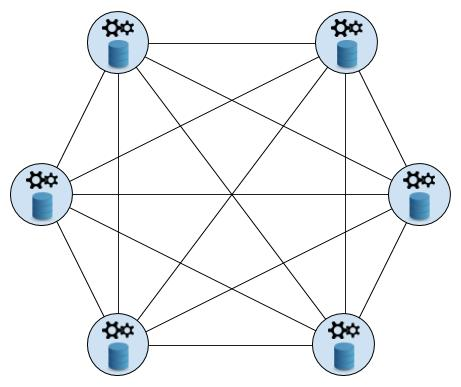
\includegraphics[width=0.6\linewidth]{figures/network_topology.jpg}
	\caption{Topologia da rede do \textit{benchmark} com $N=6$}
	\label{topologia}
\end{figure}




\label{testes}

\section{Resultados dos testes e sua discussão}


Dada a complexidade e as dificuldades associadas ao teste de
protocolos distribuídos para controlo de equipamentos de rede num
contexto real, é comum recorrer a emulação para teste dos mesmos. Os
primeiros emuladores recorriam a máquinas reais, interligadas através
de um sistema de emulação do tempo de trânsito e da perda de pacotes
numa rede real [ModelNet].

Tal como discutido em \ref{introducao}






\label{relacionado}

\section{Trabalho relacionado} \label{relac}

{ \color{blue} Apresentar outros estudos assim como técnicas usadas
fazer referência breve a ModelNet, PlanetLab, Mininet, ... estudos parecidos}

\label{fim}

\section{Conclusões e trabalho futuro}



%Surgiram alguns percalços nomeadamente na utilização do motor de base de dados, pois sabendo que os \textit{benchmarks} são testes de performance, há uma necessidade de otimizar o motor de base de dados de forma a introduzir o menor \textit{overhead} possível, pois o objectivo em questão é verificar a performance da emulação do sistema consoante as variáveis mencionadas em \ref{benchs} e evitar um \textit{bottleneck} comum entre os testes. 

%Foi discutido o aumento do número de \textit{threads} de escrita na base de dados visando melhorias ao nível do paralelismo, mas a ideia acabou por ser descartada, devido ao número de núcleos lógicos atribuído a cada máquina virtual ser único a partir de 24 instâncias. O maior imprevisto que pode ser tido em conta num trabalho futuro, surgiu aquando dos testes nas máquinas virtuais, em que, na fase de sincronização (ver \ref{func}), cada máquina virtual demorava bastante tempo (por volta de 5 minutos) a establecer as conexões para as restantes instâncias. Após algum aprofundamento da questão, chegou-se à conclusão de que estava relacionado com a resolução de nomes das restantes máquinas. Foram implementadas algumas possíveis soluções, tais como, desativar a resolução de nomes do motor da base de dados e adicionar os endereços e os nomes ao ficheiro de resolução de nomes utilizado pelo sistema operativo, mas em nenhuma das soluções se verificou uma melhoria na situação em questão. De qualquer das formas esta questão não foi mais aprofundada pois a fase que dita a performance de um determinado teste (ciclo principal, ver \ref{func}) não é influenciada.

%Surgiram também percalços relativamente á fase de sincronização do sistema, visto que a implementação inicial permitia que instâncias começassem a executar o seu ciclo principal sem que as outras estivessem no final da fase de sincronização. Visto isto, foi implementada uma solução que emula um \textit{filesystem} partilhado entre as várias instâncias (a tabela de sincronização do \textit{master node}).



Neste projeto foram avaliadas duas soluções de emulação de sistemas distribuídos escaláveis. 
Em ambos os casos foi testada a eficiência da implementação da rede virtual através de testes 
que simulavam uma troca intensiva de mensagens pela rede. 

No ambiente de testes usado, verificou-se um comportamento semelhante das duas soluções de
virtualização quando não se utiliza a emulação da rede. Em contrapartida, quando esta emulação
é usada, as VMs têm um desempenho superior quando o número de nós aumenta. A explicação deste resultado
necessita de ser aprofundada, mas tal não nos impede de retirar desde já várias conclusões imediatas.

Para começar, é importante frisar que o desenvolvimento do projeto provou ser mais ágil na plataforma Docker. 
Em contraste, no ambiente de VMs foi necessário criar vários \textit{scripts} auxiliares para
automatizar o processo de instalação e de realização dos testes.

No decorrer do desenvolvimento foram estudadas e testadas várias ferramentas disponibilizadas pelas plataformas, 
como por exemplo Docker Swarm, Docker Compose, bem como o sistema de operação 
Photon OS da VMWare. 
No entanto, estas ferramentas não foram utilizadas pois foi possível alcançar um controlo mais fino através de soluções
específicas desenvolvidas por nós.

Surgiram obstáculos relativos á utilização do MySQL devido á natureza  ACID
das transações, o que provocou um \textit{bottleneck} na utilização do disco.
Foi discutido o aumento do número de \textit{threads} de escrita na base de dados visando melhorias do desempenho. No entanto,
a ideia foi descartada 
devido ao facto de que o número de \textit{threads} total ser já consideravelmente maior que o número de núcleos do processador. 
Visto que a persistência da base de dados não era um fator importante, 
foi utilizado um \textit{ramdisk} com o objetivo de remover este \textit{bottleneck}.

Um outro imprevisto surgiu na fase de sincronização das máquinas virtuais que
demorava cerca de 40 vezes mais do que no 
Docker, devido a problemas na resolução de nomes.
Este imprevisto resultou no atraso da obtenção de resultados na fase mais crítica do trabalho.

Existe lugar para trabalho futuro imediato, nomeadamente testar os {\conts} sobre PhotonOS
e sem VM intermédia. Estes testes permitirão aprofundar a origem do \textit{overhead} suplementar verificado,
assim como aclarar a problemática da viabilidade da plataforma Docker com ou sem isolamento forte.
Relativamente às ferramentas desenvolvidas, a documentação das mesmas deve ser melhorada antes de as
disponibilizarmos publicamente. Adicionalmente, a bateria de testes poderá também ser alargada de modo a
clarificar o comportamento do sistema quando o desvio do tempo de execução começa a aumentar.

Tal como alertados pelos orientadores, a investigação em sistemas reveste-se de inúmeros obstáculos
e problemas concretos a resolver, antes de se chegarem a conclusões credíveis e verificáveis publicamente
sobre o comportamento dos sistemas, o que foi para nós algo
completamente novo.


%\tiny

\bibliographystyle{abbrv}

\bibliography{bibliography}


\end{document}
